% --- SLIDE 10: USE CASES ---
\begin{frame}{Applications \& Use Cases}

    \begin{columns}[T]

        % ── Colonna SINISTRA ──
        \begin{column}{0.32\textwidth}

            \setbeamercolor{block body}{bg=colorWalking, fg=blockText}
            \setbeamercolor{block title}{bg=colorWalking!80!black, fg=white}
            \begin{block}{\small Prosthetic Feet}
                \footnotesize \textit{(Transtibial / Transmetatarsal)}\\[0.2em]
                Passive stiffness tuning across all prosthesis levels — from partial foot to transtibial. \textbf{No electronics}, no recalibration required.
            \end{block}

            \vspace{\fill}
            \vspace{0.15cm}

            \setbeamercolor{block body}{bg=colorTerrain, fg=blockText}
            \setbeamercolor{block title}{bg=colorTerrain!80!black, fg=white}
            \begin{block}{\small Smart Insoles}
                \footnotesize \textit{(Runners / Astronauts)}\\[0.2em]
                Adaptive heel cushioning for \textbf{intact limbs}: terrain-blind impact absorption in high-load or \textit{microgravity} re-adaptation contexts.
            \end{block}

        \end{column}
        
        % ── Colonna CENTRALE (foto) ──
        \begin{column}{0.34\textwidth}
            \vspace{0.3cm}
            \begin{center}
                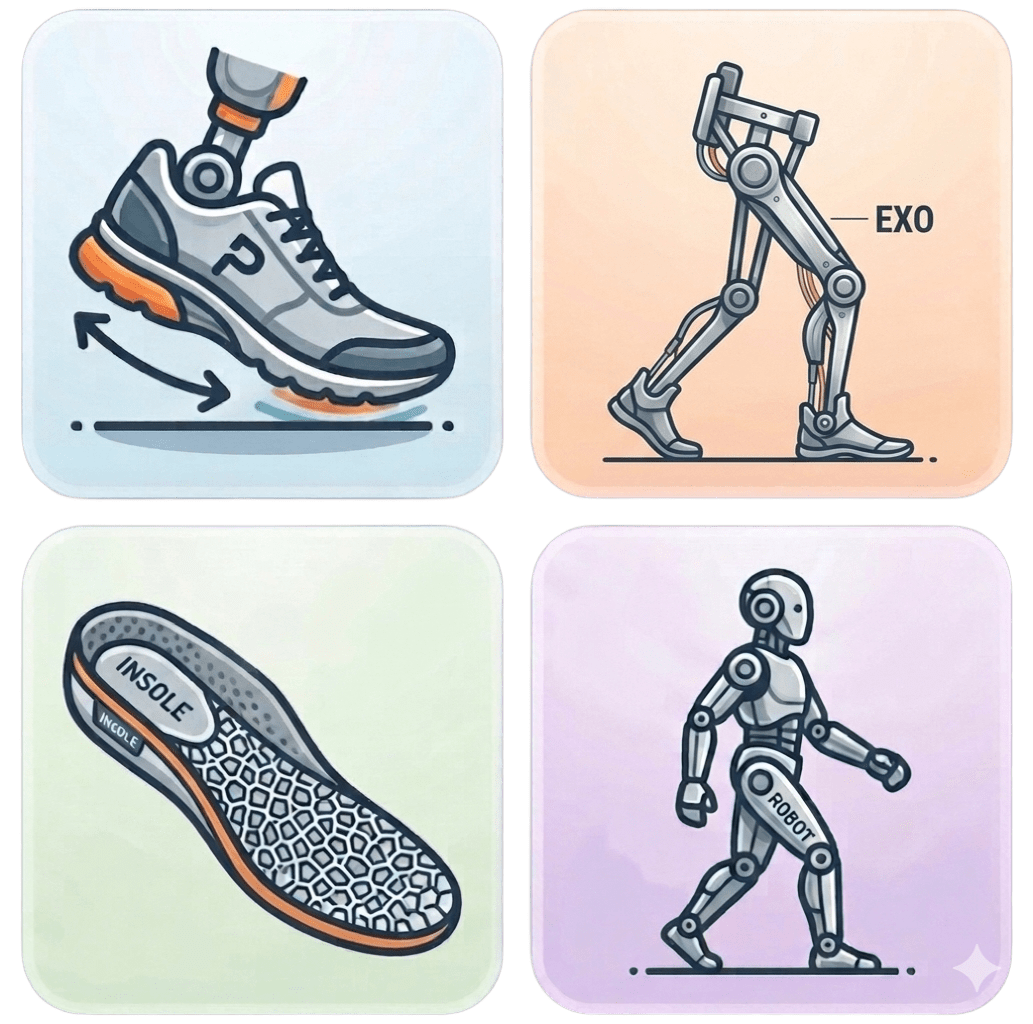
\includegraphics[width=\linewidth, height=4.8cm, keepaspectratio]{image/usecases.png}
            \end{center}
        \end{column}

        % ── Colonna DESTRA ──
        \begin{column}{0.32\textwidth}

            \setbeamercolor{block body}{bg=colorRunning, fg=blockText}
            \setbeamercolor{block title}{bg=colorRunning!80!black, fg=white}
            \begin{block}{\small Exoskeletons}
                \footnotesize \textit{(Rehabilitation / Industrial)}\\[0.2em]
                Compliant heel module for lower-limb exoskeletons: impact attenuation at \textbf{Heel Strike} without added actuators or control loops.
            \end{block}

            \vspace{0.15cm}

            \setbeamercolor{block body}{bg=colorAccess, fg=blockText}
            \setbeamercolor{block title}{bg=colorAccess!80!black, fg=white}
            \begin{block}{\small Bipedal Robots}
                \footnotesize \textit{(Humanoid / Legged Systems)}\\[0.2em]
                Passive heel compliance reduces \textbf{Ground Reaction Force} peaks at Heel Strike — no sensors, no control overhead.
            \end{block}

        \end{column}

    \end{columns}

    \vspace{0.15cm}
    \centering

\end{frame}